\section*{Quantum Harmonic Oscillator with DMC}
First of all the Hamiltonian is given by (Assuming 1D for simplicity, but it can be easily modified for 3D)
\begin{equation}
\hat{H}=- \frac{\hbar^2}{2 m}\frac{\partial^2}{\partial x^2}+\frac{1}{2}m \omega^2 x^2.
\end{equation}
Using natural units where $\hbar=1, \omega=1, m=1$ and energy is measured in units of $\hbar \omega$, this gives
\begin{equation}
\hat{H}=- \frac{1}{2}\frac{\partial^2}{\partial x^2}+\frac{1}{2}x^2.
\end{equation}
Since I know the answer I can use the exact wave function as my trial wave function.
\begin{equation}
  \Psi_T(x)=\pi^{-1/4}\exp{(-\frac{x^2}{2})}
\end{equation}
Using the above equations this gives us
\begin{equation}
  \begin{split}
    v_D &= \Psi_T^{-1}\frac{\partial}{\partial x} \Psi_T = -x \\
    E_L &= \Psi_T^{-1}\hat{H}\Psi_T = \frac{1}{2}
  \end{split}
\end{equation}
Figure~\ref{fig:1dho} shows the results for a DMC calculation of a 1-d harmonic oscillator. The exact energy for the 1-d oscillator is $E=\frac{1}{2}\hbar\omega$. The DMC energy for the calculation described in figure~\ref{fig:1dho} was $E=0.49\hbar\omega$.
\begin{figure}[h!]
  \centering
    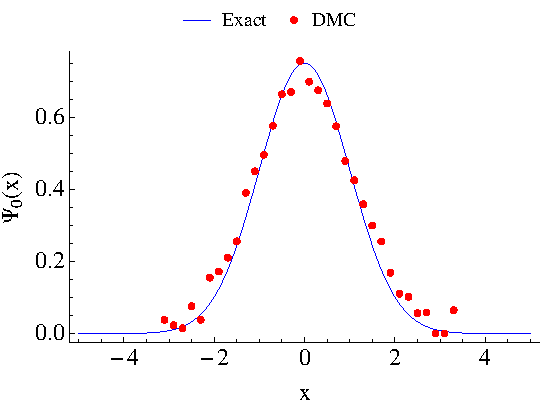
\includegraphics[width=0.5\textwidth]{notexact}
    \caption{DMC results for 1-d harmonic oscillator. Number of initial walkers was 10000, time step was 0.01, and number of time steps was 500. The exact energy is $E=\frac{1}{2}\hbar\omega$ and the DMC energy was $E=0.49\hbar\omega$.}
    \label{fig:1dho}
\end{figure}
I also did a calculation for a particle in a potential $V(x)=\frac{1}{2}x^4$, using the exact solution for the harmonic oscillator as the trial wave function. The DMC energy for this calculation was $E=0.57\hbar\omega$, and the resulting ground state wave function is shown in figure~\ref{fig:1dho4}.
\begin{figure}[h!]
  \centering
    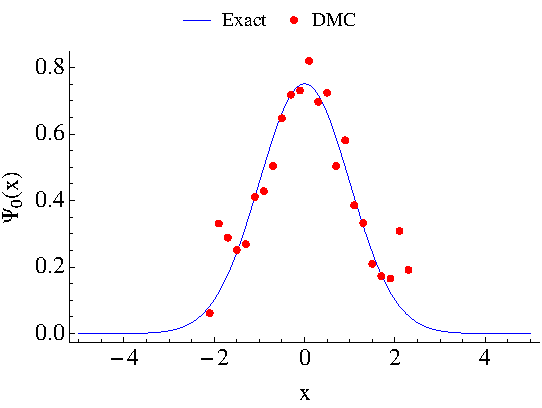
\includegraphics[width=0.5\textwidth]{notexact4}
    \caption{DMC results for particle in an $x^4$ potential. Number of initial walkers was 1000, time step was 0.01, and number of time steps was 500. The DMC energy was $E=0.57\hbar\omega$. The exact solution in this case represents the exact solution for the quantum harmonic oscillator.}
    \label{fig:1dho4}
\end{figure}
